\subsection{BoolQ Binary Classification Experiment}
Based on the BoolQ dataset \ph{[ref]} provided by Google, this experiment is designed to assess the performance of LLMs in binary classification tasks.

\subsubsection{Experimental Setup}

The Google BoolQ dataset \ph{[ref]} was utilised, containing a total of 15,942 instances. Each instance comprises three core features: a textual question, a binary answer, and a contextual passage (serving as evidence to support the answer).

The present dataset is employed for the purpose of evaluating the binary classification capabilities of Large Language Models (LLMs). The methodology employed is composed of three distinct response-style prompts, each of which is paired with a specific data parsing and post-processing pipeline.

\paragraph{LLM Judge Prompt}

The system prompt designed for the LLM is as follows:

\begin{verbatim}
"You are an assistant specialized in logical verification based on provided text. You must perform logical reasoning strictly according to the content in the Passage to analyze the binary inquiry in the Question and determine whether it aligns with the provided Answer."
\end{verbatim}

\subparagraph{Direct Mode: Binary Response Pattern}
In this mode, the Large Language Model (LLM) is required to respond exclusively with either 'true' or 'false', with no additional output permitted. The restriction of the model to a simple binary token output effectively transforms the LLM into a prompt-based binary text classifier.

This approach is specifically designed to maximise the suppression of statistical cumulative instability inherent in the auto-regressive architecture of LLMs.

\begin{placeholderblock}
[这里插入一段简单的，累乘高概率最后变成低概率的数学公式]
\end{placeholderblock}
\begin{verbatim}
# Instructions
Please perform your reasoning strictly according to these steps:
1. Analyze the logic within the "Passage," which serves as the sole basis for reasoning the answer to the "Question."
2. Derive an answer to the "Question" exclusively based on the "Passage."
3. Compare your result with the "Human Judgment Answer" to determine its correctness.

Strict Constraint: Output ONLY 'true' (if the answer is correct) or 'false' (if the answer is incorrect). Do not provide any additional information or explanation.
\end{verbatim}

\subparagraph{SSE Mode: HTTP SSE-Inspired Output Pattern}
This mode allows the LLM to output answers in a simplified format without the strict syntactical overhead of JSON, thereby preventing the unnecessary allocation of computational resources to structural formatting. The required output format is defined as:
$$
answer: boolean\\
reason: string
$$
This format is inherently human-centric, offering high readability. By enabling the reason field within this mode, we facilitate a deeper interpretability analysis of the LLM's underlying decision-making logic.

We normalize the LLM's output using the following prompt:
\begin{verbatim}
# Output Format
Please strictly follow the format below and do not include any extraneous content:

reason: 1. Cause: ..., Outcome: ...; 2. Cause: ..., Outcome: ...
answer: [True / False]
\end{verbatim}

\subparagraph{JSON Mode: Generalised Structured Output Pattern}
This mode is considered to represent the industry standard for the transformation of Large Language Models into functional "Work Models" \ph{[ref]}. In JSON mode, the LLM is required to encapsulate both the reason and the answer within a structured JSON format to facilitate seamless programmatic parsing.

With regard to universal compatibility, the methodology employed involves the configuration of the API parameter to \texttt{response\_format = json\_object}in conjunction with the implementation of robust regular expression (Regex) adaptation. This is a consequence of the inconsistent output behaviours exhibited by different models. While some models generate raw JSON strings, others wrap the content in Markdown code blocks (e.g., \texttt{\`\`\`json\textbackslash n\{json string\}\textbackslash n\`\`\`}). The experimental pipeline has been designed to dynamically adapt to these variations in order to ensure data integrity.

The following prompt is employed to standardise the LLM's output:
\begin{verbatim}
# Output Format (JSON)
You must output a valid JSON object:
```json
{
"reason": "1. Cause: ..., Outcome: ...; 2. Cause: ..., Outcome: ...; ......",
"answer": <boolean>
```
answer true: Indicates that the Human Judgment label is logically sound and correctly reflects the relationship between the passage and the question.

answer false: Indicates a contradiction or an error within the Human Judgment annotation, suggesting the label is inconsistent with the provided evidence.
\end{verbatim}

\subsubsection{Data Pre-processing and Quality Control}

Following a manual inspection, it was determined that the original dataset could not be utilised directly due to the presence of contentious samples. These problematic entries are typically categorised into two main types: non-binary responses, where the question cannot be answered with a simple true/false, and irrelevant context, where the question is decoupled from the provided passage.

In order to guarantee the validity of the evaluation, a hybrid cleaning pipeline was implemented. The process entails the implementation of a preliminary filtration procedure, which is based on the LLM. This is followed by a meticulous, item-by-item audit of the candidates that have been filtered. The aforementioned controversial instances were then consolidated into a single file, designated as dirty\_data.jsonl. During the subsequent testing phase, this "exclusion list" was loaded to ensure that the benchmarks were conducted exclusively on the refined "clean" dataset.
\begin{placeholderblock}
[这里插入争议数据集分类类别数据表]
\end{placeholderblock}

\subsubsection{Experimental parameters}

In the present experiments, a range of metrics were incorporated with a view to providing a comprehensive evaluation. The primary metric utilised to evaluate the accuracy of the results is based on the "true" or "false" tokens returned by the Large Language Model. Concurrently, the log-probabilities (logprobs) were requested from the API server to serve as a quantitative measure of model confidence.The experimental results are structured and stored as an array of tuples, defined as follows:
$$
\mathcal{D} = \{ (a_i, p_i, r_i) \}_{i=1}^N
$$
Specifically，$\mathcal{D}$ denote the experimental result set，where 
\textbf{$N$ represents the total number of questions within the BoolQ Dataset} 

For each instance $i$ ，$a_i$ is the boolean answer，$p_i$ is the maximum log-probability associated with that answer, and $r_i$ is the generated explanation.
Notably, the $r_i$ component is optional in SSE and JSON modes, whereas it is non-existent (null) in Direct mode.

To evaluate a specific LLM, we perform an instance-by-instance assessment across the entire cleaned dataset, calculating the accuracy by verifying the alignment between the model's responses and the ground truth. Furthermore, we employ $p_i$ for threshold-based filtering. Given a threshold $t$, we exclude entries where $p_i \leq t$. We then calculate both the filtered accuracy and the data retention rate (the percentage of filtered instances relative to the total dataset size).

The filtering logic is formulated as follows:
$$
\mathcal{D}_t = \{(a_i,p_i) \in \mathcal{D} | p_i \leq t\}
$$

The evaluation metrics are defined as follows:
Accuracy after filtering at threshold $t$:
$$
Acc(t) = \frac{\sum_{(a_i, p_i, r_i) \in \mathcal{D}_t} a_i}{|\mathcal{D}_t|}
$$

Data retention rate at threshold $t$:
$$
Rate(t) = \frac{|\mathcal{D}_t|}{N}
$$

\subsubsection{Implementation Details}

The following section details the implementation process.
For the purposes of this study, Python was employed as the primary programming language for the experiments, with an asynchronous programming model (asyncio) being utilised to achieve high-concurrency calls to the Large Language Model (LLM) APIs. The experimental framework is comprised of the following core components:

\paragraph{The process of loading and managing data sets}

The Hugging Face datasets library was utilised to load the Google BoolQ dataset. The DatasetManager component provides support for three distinct data split modes: train, validation, and all. In order to implement robust filtration of "dirty data," a SHA-256 hash value is computed for each individual data entry.
$$
hash_i = SHA256(question_i || passage_i || answer_i)
$$
By referencing a pre-annotated hash list of "dirty data," the framework automatically bypasses unqualified data entries during the iteration process.

\paragraph{Concurrency Control and Request Management}
To optimize API throughput while ensuring compliance with rate limits, we implemented a semaphore mechanism to regulate the maximum number of concurrent requests, which is set to a default of 10. Simultaneously, we developed an exponential backoff retry strategy to handle transient API errors, formulated as:
$$
delay_k = t_{base} \times 2^k
$$
where $t_{base}$ represents the base retry latency (defaulting to 5 seconds) and $k$ denotes the current retry attempt. The maximum number of retries is capped at 5. Our system is configured to handle various retryable error types, including rate limits (HTTP 429), server-side errors (500, 502, 503, 504), as well as timeouts and connection disruptions.

\paragraph{LLM Client Encapsulation}
The LiteLLM interface was employed as a unifying element for LLM invocations, thereby enabling seamless transitions between various API providers, including OpenRouter and Google Vertex AI. In the context of the Gemini model series, the Google GenAI SDK has been integrated with a specific objective in mind: to capitalise on the inherent support for log-probabilities (logprobs) within the framework. In order to monitor performance, the client logs the initiation timestamp of each request and calculates the inference latency upon receiving the response:
$$
latency_i = t_{response} - t_{request}
$$

\paragraph{Response Parsers}

Specifically, a range of response parsing strategies was implemented, with each tailored for one of the three distinct output formats.

\begin{itemize}
\item \textbf{DirectModeParsing}:The utilisation of regular expressions (Regex) is employed for the purpose of matching standalone word boundaries for the values \texttt{\textbackslash btrue\textbackslash b} or \texttt{\textbackslash bfalse\textbackslash b}
\item \textbf{SSEModeParsing}:Regex is employed to extract fields that match the given pattern:\texttt{answer:\textbackslash s*(true|false)}
\item \textbf{JSONModeParsing}:The system under discussion has the capacity to support both raw JSON strings and JSON objects that are encapsulated within code blocks that are denoted by the characters "\texttt{json}". The system extracts the JSON object by locating the first occurrence of \texttt{\{}and the final occurrence of \texttt{\}}.
\end{itemize}

In order to mitigate the occurrence of occasional formatting irregularities, the system has been programmed to automatically perform up to two retries upon the occurrence of a parsing failure, thus ensuring a higher degree of data reliability.

\paragraph{LogProbs Collection and Confidence Quantification}
In the context of our API requests, the logprobs parameter is enabled, and top\_logprobs=5 is set to capture the top five candidate probabilities for each output token. For each response, the log-probabilities of all generated tokens are aggregated and their arithmetic mean is computed.
$$
\bar{p}_i = \frac{1}{|T_i|} \sum_{t \in T_i} \log P(t)
$$
In this context, $T_i$ is used to denote the token sequence of the $i$-th response. The final confidence score is then derived via an exponential transformation of the average log-probability:
$$
confidence_i = e^{\bar{p}_i}
$$

\paragraph{Cost Estimation}
The completion\_cost function from the LiteLLM library was utilised to perform real-time cost accounting. For models not natively supported by the library, an internal fallback pricing table has been implemented. The cost analysis encapsulates input token expenses, output token expenses, and the total expenditure, providing both real-time monitoring and projected total costs for the entire experimental run.

\paragraph{Data Persistence and Logging}
The experimental results are streamed in real-time to JSONL (JSON Lines) files via an AsyncResultWriter, ensuring data integrity during high-concurrency execution. Each record is characterised by its high level of granularity, with the following fields incorporated:(这里ai自动分类了子项)
Contextual Data: Question, Passage, and Index.

Model Performance: The following three elements are to be considered: human judgment (ground truth), predicted answer and correctness.

Reasoning \& Meta-data: The following elements are to be considered: raw response, parsed reasoning, inference latency and timestamp.

Probabilistic and Statistical Data: The following data is to be provided: a SHA-256 hash, average log-probabilities, confidence scores and the complete log-probabilities distribution list.

The utilisation of resources is as follows: The utilisation of tokens and the associated financial expenditure.

Concurrently, comprehensive experimental logs are stored in independent .log files, featuring detailed execution statistics and log-probability distribution histograms for diagnostic analysis.

\subsubsection{Main Results}

\begin{figure}[htbp]
\centerline{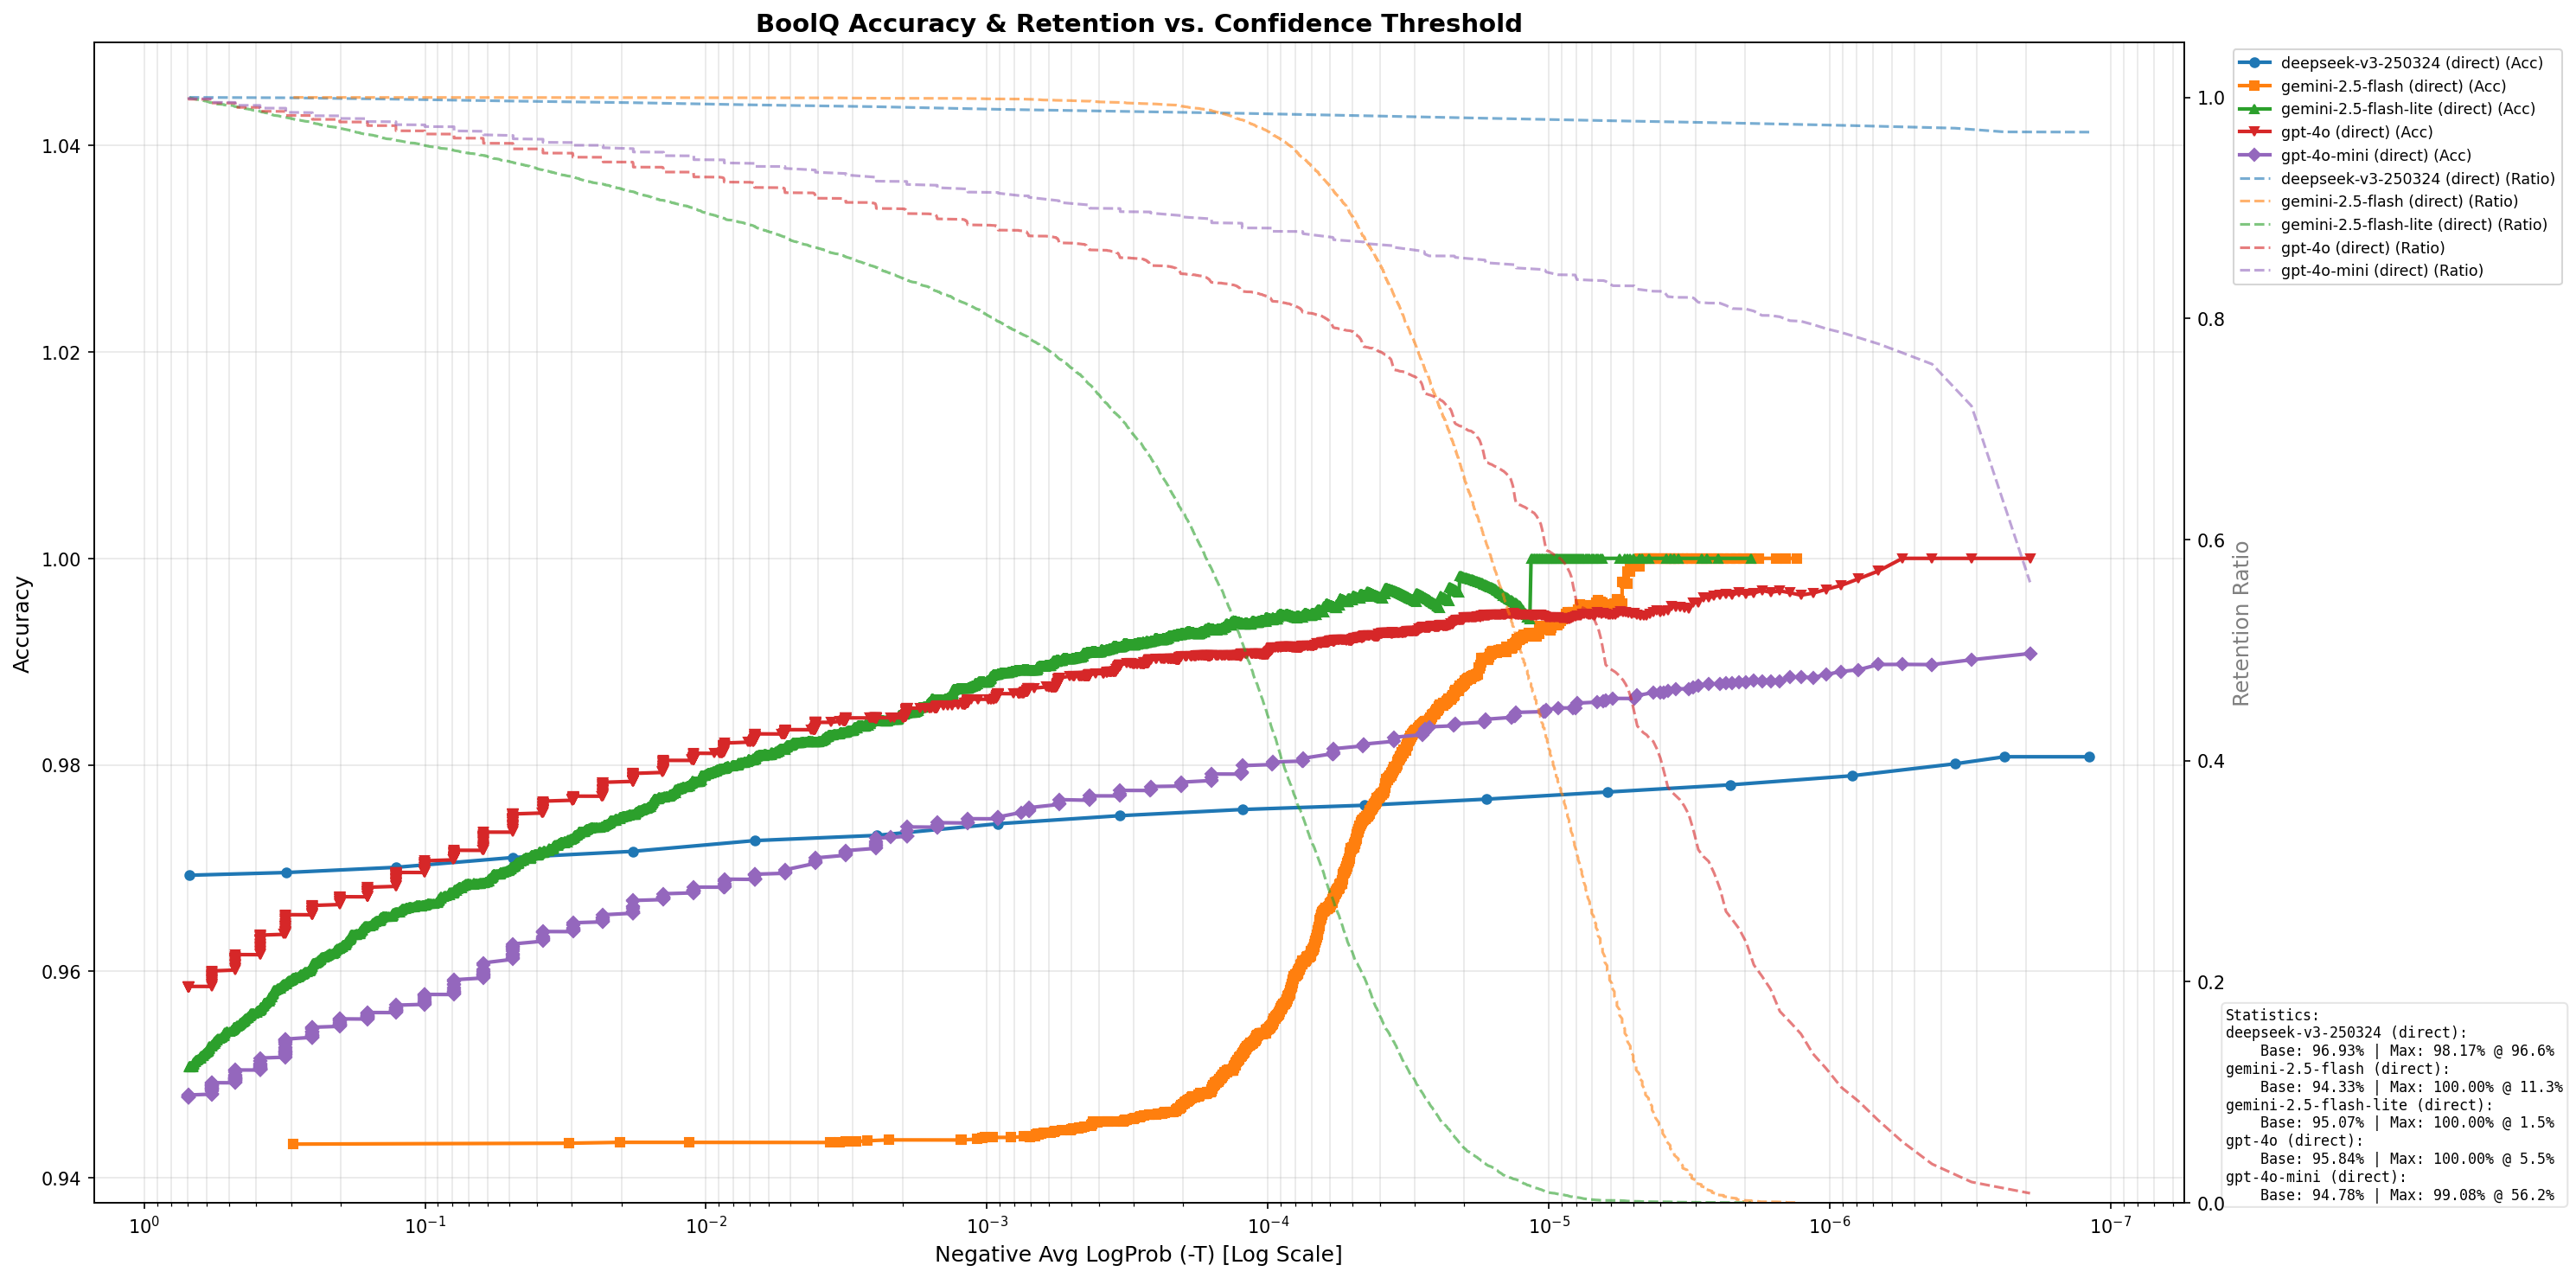
\includegraphics{../../BoolQuestion_LLM_Test/outputs/images/accuracy_vs_logprob.png}}
\caption{Accuracy vs Logprobs Threshold}
\label{fig:boolq_results}
\end{figure}

An evaluation of five state-of-the-art Large Language Models (LLMs) in Direct Mode was conducted. The following devices are under consideration: DeepSeek-V3, Gemini-2.5-Flash, Gemini-2.5-Flash-Lite, GPT-4o and GPT-4o-mini.The solid lines in the figure represent the accuracy curves across varying logprobs thresholds, while the dashed lines denote the corresponding data retention rates.

\paragraph{Key Findings: High Reliability of LLMs as Binary Classifiers}
The experimental results provide compelling evidence for the reliability of Large Language Models in binary classification tasks. In the absence of any confidence-based filtering, \textbf{all tested models achieved a baseline accuracy exceeding 94\%}.
Specifically, the model DeepSeek-V3 demonstrated the most proficient performance with a baseline accuracy of\textbf{96.93\%}, closely followed by GPT-4o with 95.84\%. Meanwhile, Gemini-2.5-Flash-Lite attained 95.07\%. The findings indicate that contemporary state-of-the-art LLMs possess the fundamental capability to serve as reliable decision-making components within automated workflows. Despite the absence of confidence-based screening, the error rates remained within the range of 3\% and 6\%.

\paragraph{Significant Performance Gains from Confidence-based Filtering}

The implementation of the logprobs threshold filtering mechanism has been demonstrated to engender substantial enhancements in the binary classification performance of LLMs. The performance of DeepSeek-V3 is particularly noteworthy: under a lenient filtering condition that retains \textbf{96.6\%}of the data, its accuracy improves from 96.93\% to \textbf{98.17\%}. This suggests that the filtration of a mere 3.4\% of low-confidence samples can yield an accuracy gain of over 1.2 percentage points, with negligible loss in data coverage for real-world applications.

It is evident from the observation of the morphology of the retention curves that DeepSeek-V3 consistently maintains a retention rate that is above 96\% across the entire threshold range. This finding suggests that the model's confidence distribution is predominantly concentrated within the high-confidence interval, indicating a more rational internal uncertainty distribution. This characteristic is of significant practical value in automated scenarios that demand a balance between \textbf{accuracy} and \textbf{data coverage}.

As demonstrated in Figure~\ref{fig:boolq_results}, GPT-4o-mini also exhibits excellent results, achieving an accuracy of \textbf{99.08\%} while retaining \textbf{56.2\%} of the data. In scenarios requiring extreme precision, GPT-4o attains \textbf{100\%} accuracy while retaining the top 5.5\% most confident samples, and Gemini-2.5-Flash attains the same 100\% mark at an 11.3\% retention rate. Despite the reduced data retention in these cases, the system provides a viable solution for zero-tolerance, mission-critical decision-making processes.

\paragraph{Implications for Automated Workflows}
The empirical findings of this study offer significant insights for the integration of Large Language Models within automated production pipelines:
\begin{enumerate}
\item \textbf{Out-of-the-box Reliability}：A baseline accuracy that exceeds 94\% indicates that LLMs can be directly deployed as binary decision-making components in automation. This level of performance has been demonstrated to meet the reliability requirements of the majority of application scenarios, thus obviating the necessity for additional calibration or fine-tuning.
\item \textbf{Flexible Accuracy-Coverage Trade-off}：It is possible to dynamically configure the balance between precision and data coverage by tuning the logprobs threshold. This can be done in order to align with specific business objectives or risk tolerances.
\item \textbf{High-Efficiency Confidence Filtering}：A prime example of this is the DeepSeek-V3, which has been shown to achieve significant accuracy gains by filtering a mere 3.4\% of samples, thus demonstrating an exceptional cost-benefit ratio. This, in turn, maximises reliability while preserving high throughput.
\end{enumerate}

In conclusion, it is evident that LLMs have attained a level of reliability as binary classifiers. Coupled with logprobs-based filtering mechanisms, they are fully qualified as robust decision-making modules for enterprise-grade automated workflows.
